%%%%%%%%%%%%%%%%%%%%%%%%%%%%%%%%%%%%%%%%%%%%%%%%%%%%%%%%%%%%%%%%%%%%%%%%%%%%%%%%%%%%%%%%%%
% Dokumenttypen Beamer låter oss skapa slides m.h.a. LaTeX
%
% I stort sett allt fungerar som ni är vana vid när det kommer till  formatering, men
% en markant skillnad är \verb som inte fungerar.  Använd i stället
% \texttt{<insert text here>}.
%
% Ny slide sätts i miljön ``frame''. Se gärna dummies och sliden i TSIU03 för basic stuff.
% Full dokumentation återfinns på:
% http://ftp.acc.umu.se/mirror/CTAN/macros/latex/contrib/beamer/doc/beameruserguide.pdf
%%%%%%%%%%%%%%%%%%%%%%%%%%%%%%%%%%%%%%%%%%%%%%%%%%%%%%%%%%%%%%%%%%%%%%%%%%%%%%%%%%%%%%%%%%

\begin{frame}
  \frametitle{Akitektur}
  \framesubtitle{Överblick -- principskiss}
  \begin{figure}
    \centering
    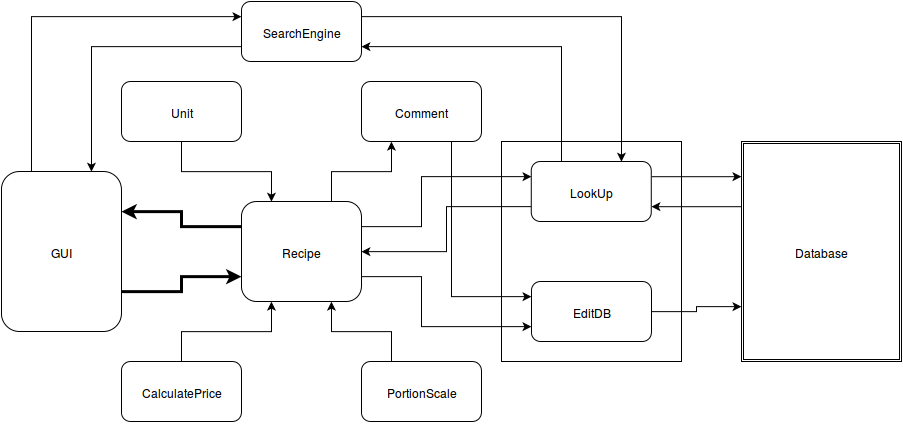
\includegraphics[scale=.3]{overview}
  \end{figure}
\end{frame}
